\documentclass[12pt,a4paper,]{scrreprt}
\usepackage[ngerman]{babel}
\usepackage[onehalfspacing]{setspace}
\usepackage[utf8]{inputenc}

\usepackage{graphicx,array,gnuplottex,siunitx,multicol,capt-of,amsmath,ulem,amsthm}
\let\phi\varphi
\setkomafont{chapter}{\fontsize{20bp}{22.2bp}\selectfont\bfseries}

\setkomafont{chapter}{\fontsize{14bp}{18.8bp}\selectfont\bfseries}
\setkomafont{section}{\fontsize{12bp}{14.4bp}\selectfont\bfseries}

\renewcommand{\chapterheadstartvskip}{\vspace*{-1\topskip}}
\renewcommand{\chapterheadendvskip}{\vspace*{0.8\topskip}}
%---------------------------------------------------------------------------------------------------------------------------------------------------------------
% Ende der Einstellungen
%---------------------------------------------------------------------------------------------------------------------------------------------------------------

%---------------------------------------------------------------------------------------------------------------------------------------------------------------
%Ab hier gibt es Inhalt
%---------------------------------------------------------------------------------------------------------------------------------------------------------------
\begin{document}

\title{Wechselstromwiderstände und Serienschwingkreis (Korrektur)}
\author{Henrik Jäger \\ 3114168 \and Lena Majer \\ 3115808}
\subtitle{E10a \\  Assistent: Wolfgang Voesch}
\subject{Physikalisches Praktikum I}
\publishers{Universität Stuttgart}
\date{24. November 2016}
%\thanks{Assistent: Sascha Kolatschek}

\maketitle% Titelei

\tableofcontents   %Inhaltsverzeichnis
\pagebreak
\chapter{Einleitung}
\section{Ziel}
In diesem Versuch geht es um die Bestimmung einem frequenzabhängigen Widerstand eines Schwingkreises. Im Laufe des Versuches wird zudem die Resonanzfrequenz bestimmt.
\section{Grundlagen}
Widerstände, die in Serie geschaltet werden, können um den Gesamtwiderstand zu bestimmen addiert werden. Die gesamte Spannung kann bei in Serie geschalteten  Widerständen ebenfalls so ermittelt werden, dass man die Spannungen, die an den einzelnen Widerständen anliegen, addiert. Der Strom durch die Einzelnen in Reihe geschalteten Widerstände ist gleich.\\
\begin{equation}
R_0= R_1 + R_2+…
\end{equation}
 \begin{equation}
 U_0 = U_1+U_2+…
 \end{equation}
 \begin{equation}
 I_0 = I_1 = I_2…
 \end{equation}
Sind Widerstände parallel geschaltet, errechnet sich eins durch den Gesamtwiderstand als Summe von eins durch die einzelnen Widerstände. Die Spannung die an einem einzelnen Wiederstand anliegt, liegt auch an allen anderen einzelnen Widerständen an. Der Gesamtstrom setzt sich aus den einzelnen Strömen durch die einzelnen Wiederstände zusammen.\\
\begin{equation}
\frac{1}{R_0} = \frac{1}{R_1} + \frac{1}{R_2} ...
\end{equation}
\begin{equation}
 U_0 = U_1 = U_2 …
\end{equation}
\begin{equation}
 I_0 = I_1 + I_2 + …
\end{equation}
Besitzt eine Schaltung nicht nur Widerstände und stattdessen auch Spulen und Kondensatoren muss auch beachtet werden, dass Spulen und Kondensatoren unterschiedliche Verhaltensweisen bei Wechselstrom und Gleichstrom haben. Für eine Spule gilt:\\
\begin{equation}
U=L\cdot \frac{d}{dt} I
\end{equation}
\begin{equation}
Z_L= \frac{U}{I} = i \cdot \omega \cdot L
\end{equation}
Hierbei entspricht L der Induktivität der Spule. Bei Spulen ist die Spannung um $\pi/2$ vor den Strom verschoben.\\
Für einen Kondensator gilt:\\
\begin{equation}
I = C\cdot\dot{U}
\end{equation}
 \begin{equation}
 Z_C = \frac{U}{I} = -\frac{i}{\omega \cdot C}
 \end{equation}
C entspricht der Kapazität. Bei Kondensatoren ist die Spannung um $\pi/2$ hinter den Strom verschoben.\\
Wechselströme können mithilfe imaginärer Exponentialfunktionen beschrieben werden:\\
\begin{equation}
I=I_0 \cdot \exp(i\cdot \omega \cdot t)
\end{equation}
$I_0$ entspricht der Amplitude, $\omega$ der Kreisfrequenz.\\
\pagebreak

\chapter{Messprinzip mit Skizze und Versuchsablauf}
\begin{center}
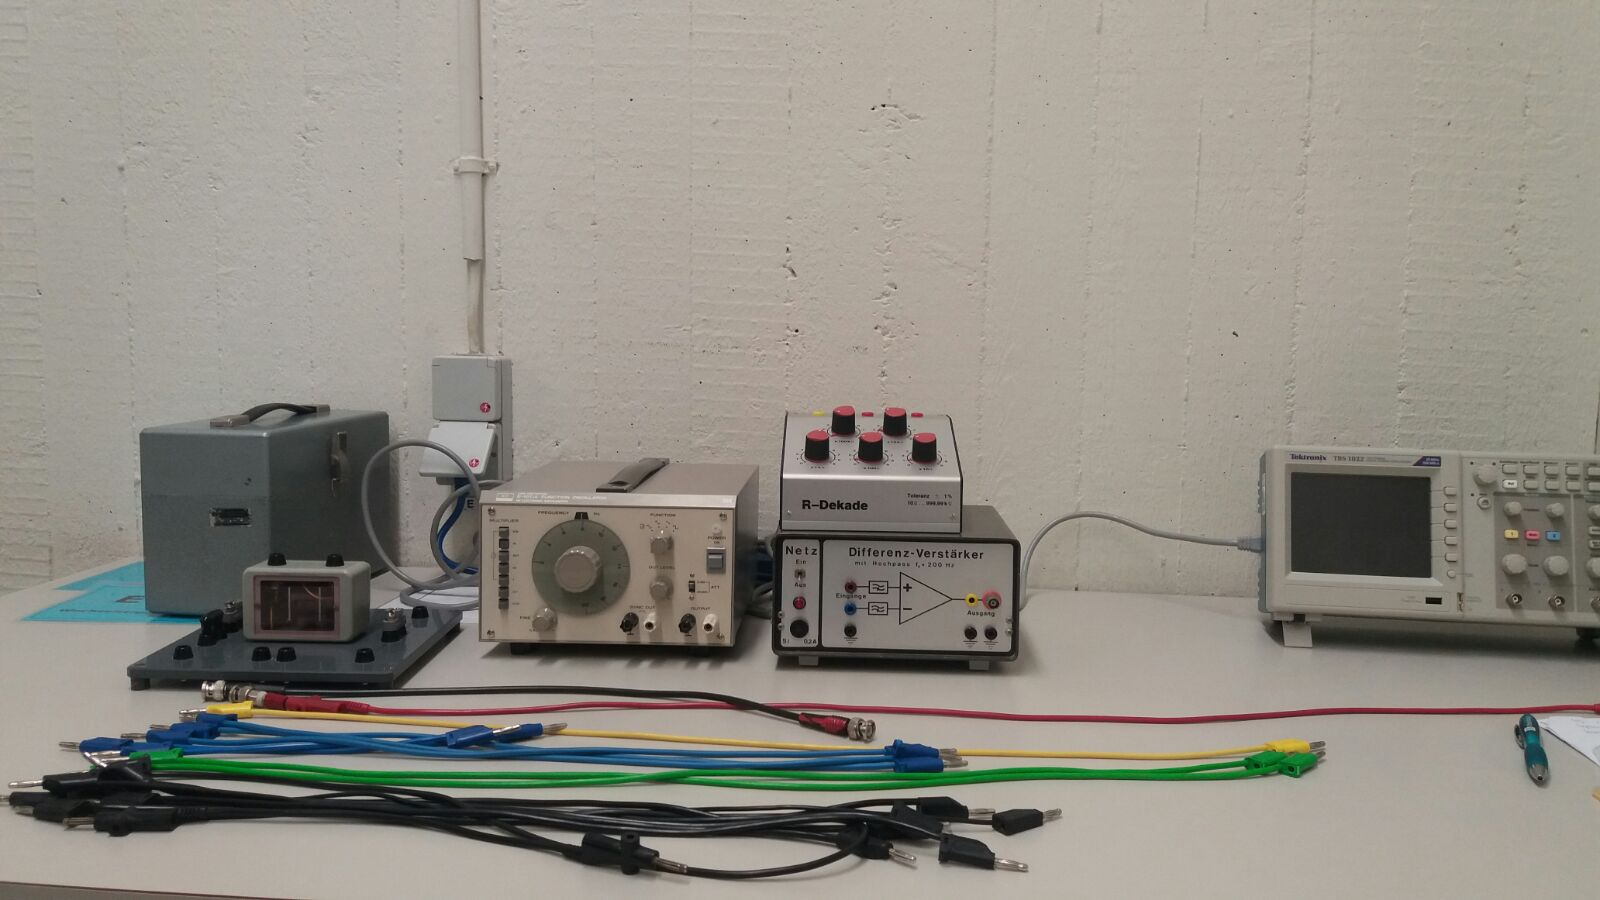
\includegraphics[scale=0.2]{Daten/aufbau.jpeg}
\end{center}
\captionof{figure}[aufbau]{Versuchsaufbau}
Nach Aufbauen der ersten Schaltung wurde zubeginn des Versuchstages zunächst grob die Resonanzfrequenz bestimmt. \\
Dazu wird eine Leitungsbrücke angewendet. Die Schaltung ist an ein Oszilloskop angeschlossen. Dierbei wird nun versucht, die Varianz der  Amplitunde des Signal möglichst zu minimieren.\\
\\
Sobald ein grober Wert der Resonanzfrequenzes des Schwingkreises bestimmt wurden ist, wird die Leitungsbrücke entfernt.\\
Nach entfernen der Leitungsbrücke werden jewils 10 Messpunkte oberhalb des groben Ressonanzwertes und jeweils 10 Messpunkte unterhalb des groben Ressonanzwertes bestimmt.\\
Dabei wird an verschiedenen Frequenzen erneut versucht, durch Regelung eines einstellbaren Widerstands und eines Kondensators, die Amplitude des Signal möglichst minimal zu bekommen. \\
Es wird ab einer Frequenz von 0,2 KHz gemessen. Die maximale Frequenz liegt bei 8 KHz. Die Messpunkte werden in der Nähe der Resonanzfrequenz näher beieinander gewählt.
	\pagebreak


	
\chapter{Formeln}
    Zur Bestimmung der Stärke des magnetischen Feldes B wird die Formel:
    \begin{equation}
		B =\frac{1}{2 \pi f \cdot n\cdot A}U_{ind}
	\end{equation}
verwendet. Hierbei beschreibt $f$ die Frequenz der Wechselspannung, $n$ die Windungszahl und A die Spulenfläche.\\
\\
Sobald eine zeitliche Änderung des Magnetischen Fusses in einer Spule vorgenommen wird entsteht eine Induktionsspannung. Hierfür gilt:\\
\begin{equation}
	\Phi=B \cdot A
\end{equation}
	
     Der ohmschen Widerstand wird über den spezifischen Widerstand $\rho_{cu}$ berechnet:\\
  \begin{equation}
    	R_{sp} =  \rho_{cu} \cdot \frac{l_{sp}}{A_{sp}}
        \label{}
  \end{equation}
  l beschreibt hierbei die Länge der Spule und A die Fläche der Spule.\\
  
  Mit $l = \pi \cdot d \cdot n_a$ und $A = \pi \cdot \frac{1}{4} d^2$ ist der Widerstand der Spule gegeben:
    \begin{equation}
    	R_{sp}=\rho\cdot\frac{\pi\cdot 2 r\cdot n_a}{\pi\cdot\frac{1}{4}\cdot d^2} = \rho\cdot\frac{8\cdot r\cdot n_a}{d^2} \\
        \label{spezifischerWiderstand}
    \end{equation}
    \\
    Die Induktivität L kann über die Spannungen bestimmt werden. Hierfür gilt:
    \begin{equation}
    L= \sqrt{\frac{U_e \cdot R}{U_a \cdot \omega^2}}
    \label{InduktivitaetSpannung}
    \end{equation}
  \\
  Mit der Formel
\begin{equation}
	f  = \frac{1}{2\pi\cdot\sqrt{ L\cdot C}}
\end{equation}
gilt für die Induktivität L der Spule:
\begin{equation}
	  L= \frac{1}{f^2 \cdot 4\pi^2 \cdot C} 
      \label{InduktivitaetFrequenz}
\end{equation}
 
        \pagebreak
    

	\chapter{Auswertung}
    	\section{Germanium- und Siliziumdioden in Durchlassrichtung}
        	\begin{gnuplot}[terminal=pdf,terminaloptions={font ",10" linewidth 2},scale=1.2]
            		set fit errorvariables
					
                  	set xlabel "Spannung [V]"
                  	set ylabel "Stromstärke [mA]"
					set xrange [0:1]
                    set yrange [0:1]
                    
                    f(x) = a*exp(b*x)
                    g(x) = c*exp(d*x)
                    fit f(x) "Daten/A1a.txt" using 2:1 via a,b
                    fit g(x) "Daten/A1a.txt" using 3:1 via c,d
                    
                  	plot "Daten/A1a.txt" using 2:1 title "Germanium", "Daten/A1a.txt" using 3:1 title "Silizium", f(x), g(x)
			\end{gnuplot}
        \captionof{figure}[DurchlassGerSil]{Kennlinien der Dioden in Durchlassrichtung}
        Im Diagramm wurde die Fitfunktion 			
        \begin{equation}
        	f(x) = a \cdot \exp(b\cdot x)
        \end{equation}
        verwendet. \\
        
        Wenn wir davon ausgehen, dass Formel \ref{Sperrstrom-vereinfacht} gilt, können wir den Sperrstrom aus den gefitteten Werten ermitteln. \\
        
        Es ergibt sich:
	\begin{center}
		\begin{tabular}{c|cc}
			&  Germanium & Silizium\\ \hline
    		$I_s$ & $0.3\cdot 10^{-3} mA$ &  $0.04\cdot 10^{-6} mA$
		\end{tabular}
    \end{center}    
   		     
        
        \pagebreak
        
        \section{Germanium- und Silizium in Sperrrichtung}
        \begin{gnuplot}[terminal=pdf,terminaloptions={font ",10" linewidth 2},scale=1.2]
        	set xlabel "Spannung [V]"
			set ylabel "Stromstärke [Mikroampere]"
            
			f(x)=a*x+b
            g(x)=c*x+d
            
            set key left
            
            set xrange [-8:0]
            
            fit f(x) "Daten/A1c.txt" using 1:2 via a,b
            fit g(x) "Daten/A1c.txt" using 1:3 via c,d
           	
            plot "Daten/A1c.txt" using 1:2 title "Germanium", "Daten/A1c.txt" using 1:3 title "Silizium", f(x), g(x)
                    
			\end{gnuplot}
        \captionof{figure}[DurchlassGerSil]{Kennlinien der Dioden in Sperrrichtung}
        
       \ \\
       Die Werte passen nicht zu den im ersten Versuchsteil bestimmten Sperrströmen
        \pagebreak
        
        \section{Zenerdiode in Durchlass- und Sperrrichtung}
        	Trägt man Durchlass und Sperrrichtungskennlinien in einem gemeinsamen Diagramm auf erhält man die Z-Linie. \\
        	\begin{gnuplot}[terminal=pdf,terminaloptions={font ",10" linewidth 2},scale=1.2]
					
                  	set xlabel "Spannung [V]"
                  	set ylabel "Stromstärke [Mikroampere]"
                  	
                  	plot "Daten/A2a.txt" using 2:1 title "Durchlassrichtung", "Daten/A2b.txt" using 1:2 title "Sperrrichtung 
			\end{gnuplot}
        \captionof{figure}[DurchlassGerSil]{Gesamtkennlinie der Zener-Diode} 
        \ \\
        Hier spielt in der Sperrrichtung die spezielle Eigenschaft der Zener-Diode eine Rolle. Ab einer gewissen Sperrspannung nimmt ihr differentieller Widerstand exponentiell zu, während er vor dieser Spannung noch nicht vorhanden war.\ \\
        Bei einer Spannung von $ U = 5,75 V$ wurde mit der $\mu A$ -Skala ein Strom von $948 \mu A$ gemessen. Mit der mA-Skala wurde aber ein Strom von $960 \mu A$ gemessen. Die $\mu A$-Skala ist auf genaueres Messen ausgelegt, während die mA-Skala höhere Ströme aushält.
        
        \pagebreak
        
        \section{LEDs mit Oszilloskop}
        \begin{center}
        
         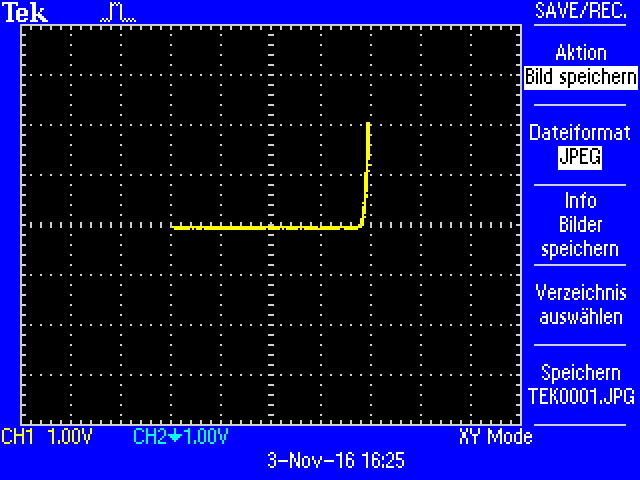
\includegraphics[scale=1]{Daten/TEK0001.JPG}
           \captionof{figure}[DurchlassGerSil]{Kennlinie der roten LED} 
         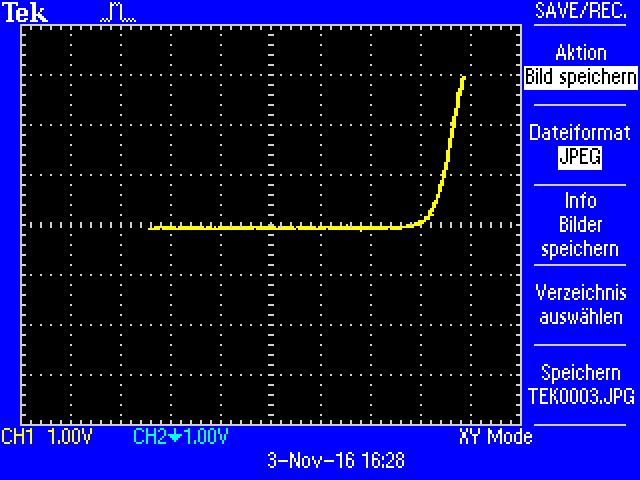
\includegraphics[scale=1]{Daten/TEK0003.JPG}
           \captionof{figure}[DurchlassGerSil]{Kennlinie der blauen LED} 
           \end{center}
        
       Die Schwellspannungen sind aus den Diagrammen abzulesen und sind:
       \begin{center}
       \begin{tabular}{c|c}
       &Schwellspannung\\ \hline
       Rot & $1,8 V$ \\
       Blau & $2,7 V$
       \end{tabular}
       \end{center}
       Damit lässt sich die Wellenlänge des Lichtes berechnen, das von der LED abgestrahlt wird.
       \begin{align*}
       		\lambda_{rot} & = \frac{h \cdot c}{e \cdot U_{rot}} \\
            & = \frac{6,626 \cdot 10^{-34} Js \cdot 0,3 \cdot 10^9 \frac{m}{s}}{1,6 \cdot 10^{-19} C \cdot 1,8 V} = 690,2 nm
       \end{align*} 
       \begin{align*}
       		\lambda_{blau} & = \frac{h \cdot c}{e \cdot U_{blau}} \\
            & = \frac{6,626 \cdot 10^{-34} Js \cdot 0,3 \cdot 10^9 \frac{m}{s}}{1,6 \cdot 10^{-19} C \cdot 2,7 V} = 460,1 nm
       \end{align*}
       
       Die errechneten Wellenlängen passen sehr gut zum Licht, dass von den LEDs abgestrahlt wird, wenn man für blaues Licht eine Wellenlänge von $420nm$ bis $490nm$ und $650nm$ bis $750nm$ für rotes Licht annimmt. \footnote{https://de.wikipedia.org/wiki/Licht}
	\pagebreak

\chapter{Fehlerbetrachtung}
	Durch die verschiedenen Werte kann man eine Abweichung von 
    \begin{align*}
    	\frac{|f_1 - f_2|}{2} = \Delta f =  \pm 16,75 Hz
    \end{align*}
    erwarten. 

    Die in diesem Versuch entstandenen Fehler erklären sich durch:
    \begin{itemize}
    \item die Ungenauigkeit der Messgeräte. Die Verwendeten Messgeräte können keine ganz genauen Daten liefern, da sie nicht mit einer absouten Genauigkeit gebaut werden können. Es treten bei allen Messgeräten Fehler auf. Es kann nur versucht werden, diese Fehler sehr klein zu halten.
    \item die Ungenauigkeit des Ablesens. Auch beim ablesen, ist die Skala nur auf einen gewissen Kommawet ablesbar. Um dort weniger Fehler erhalten zu können, müsste eine genauere Skala verwendet werden.
    \item das Rauschen. Das auf dem Oszilloskop angezeigte Signal Rauscht zum Teil sehr stark. Dies bringt einen weiteren Faktor, der es nicht ermöglicht einen Wert genau abzulessen.
    \end{itemize}
Die  ersten Messwerde wurden widerholt, da die Abweichung zu den anderen  Messwerten größer als erwartet war. Vermutlich kam die starke Abweichung durch fehlende Routine  bei den ersten Messungen. Die weiteren Messungen passten daraufhin schon deutlich besser.
	\pagebreak

	\chapter{Zusammenfassung}
    In diesem Versuch wurde zunächst Grob (durch Verwendung einer Leitungsbrücke) die Resonanzfrequenz bestimmt. \\
    Es wurde die Frequenz von 1,495 kHz ermittelt.\\
    \\
    Danach wurde durch viele Messwerte um die Resonanzfrequenz und dabei Ablesen der Kapazität und des verstellbaren Widerstands die Werte bestimmt, mit denen eine genauere Resonanzfrequenz ermittelt werden konnte.\\
    
   Hierfür wurde ein Wert von $f=(1463,25 \pm 16,75) Hz$ ermittelt.\\
   \\
   Fehlerquellen kommen durch Ableseungenauigkeiten und Ungenauigkeiten der Messgeräte.
	\pagebreak

	\section{Anhang}
    
    \begin{center}
    		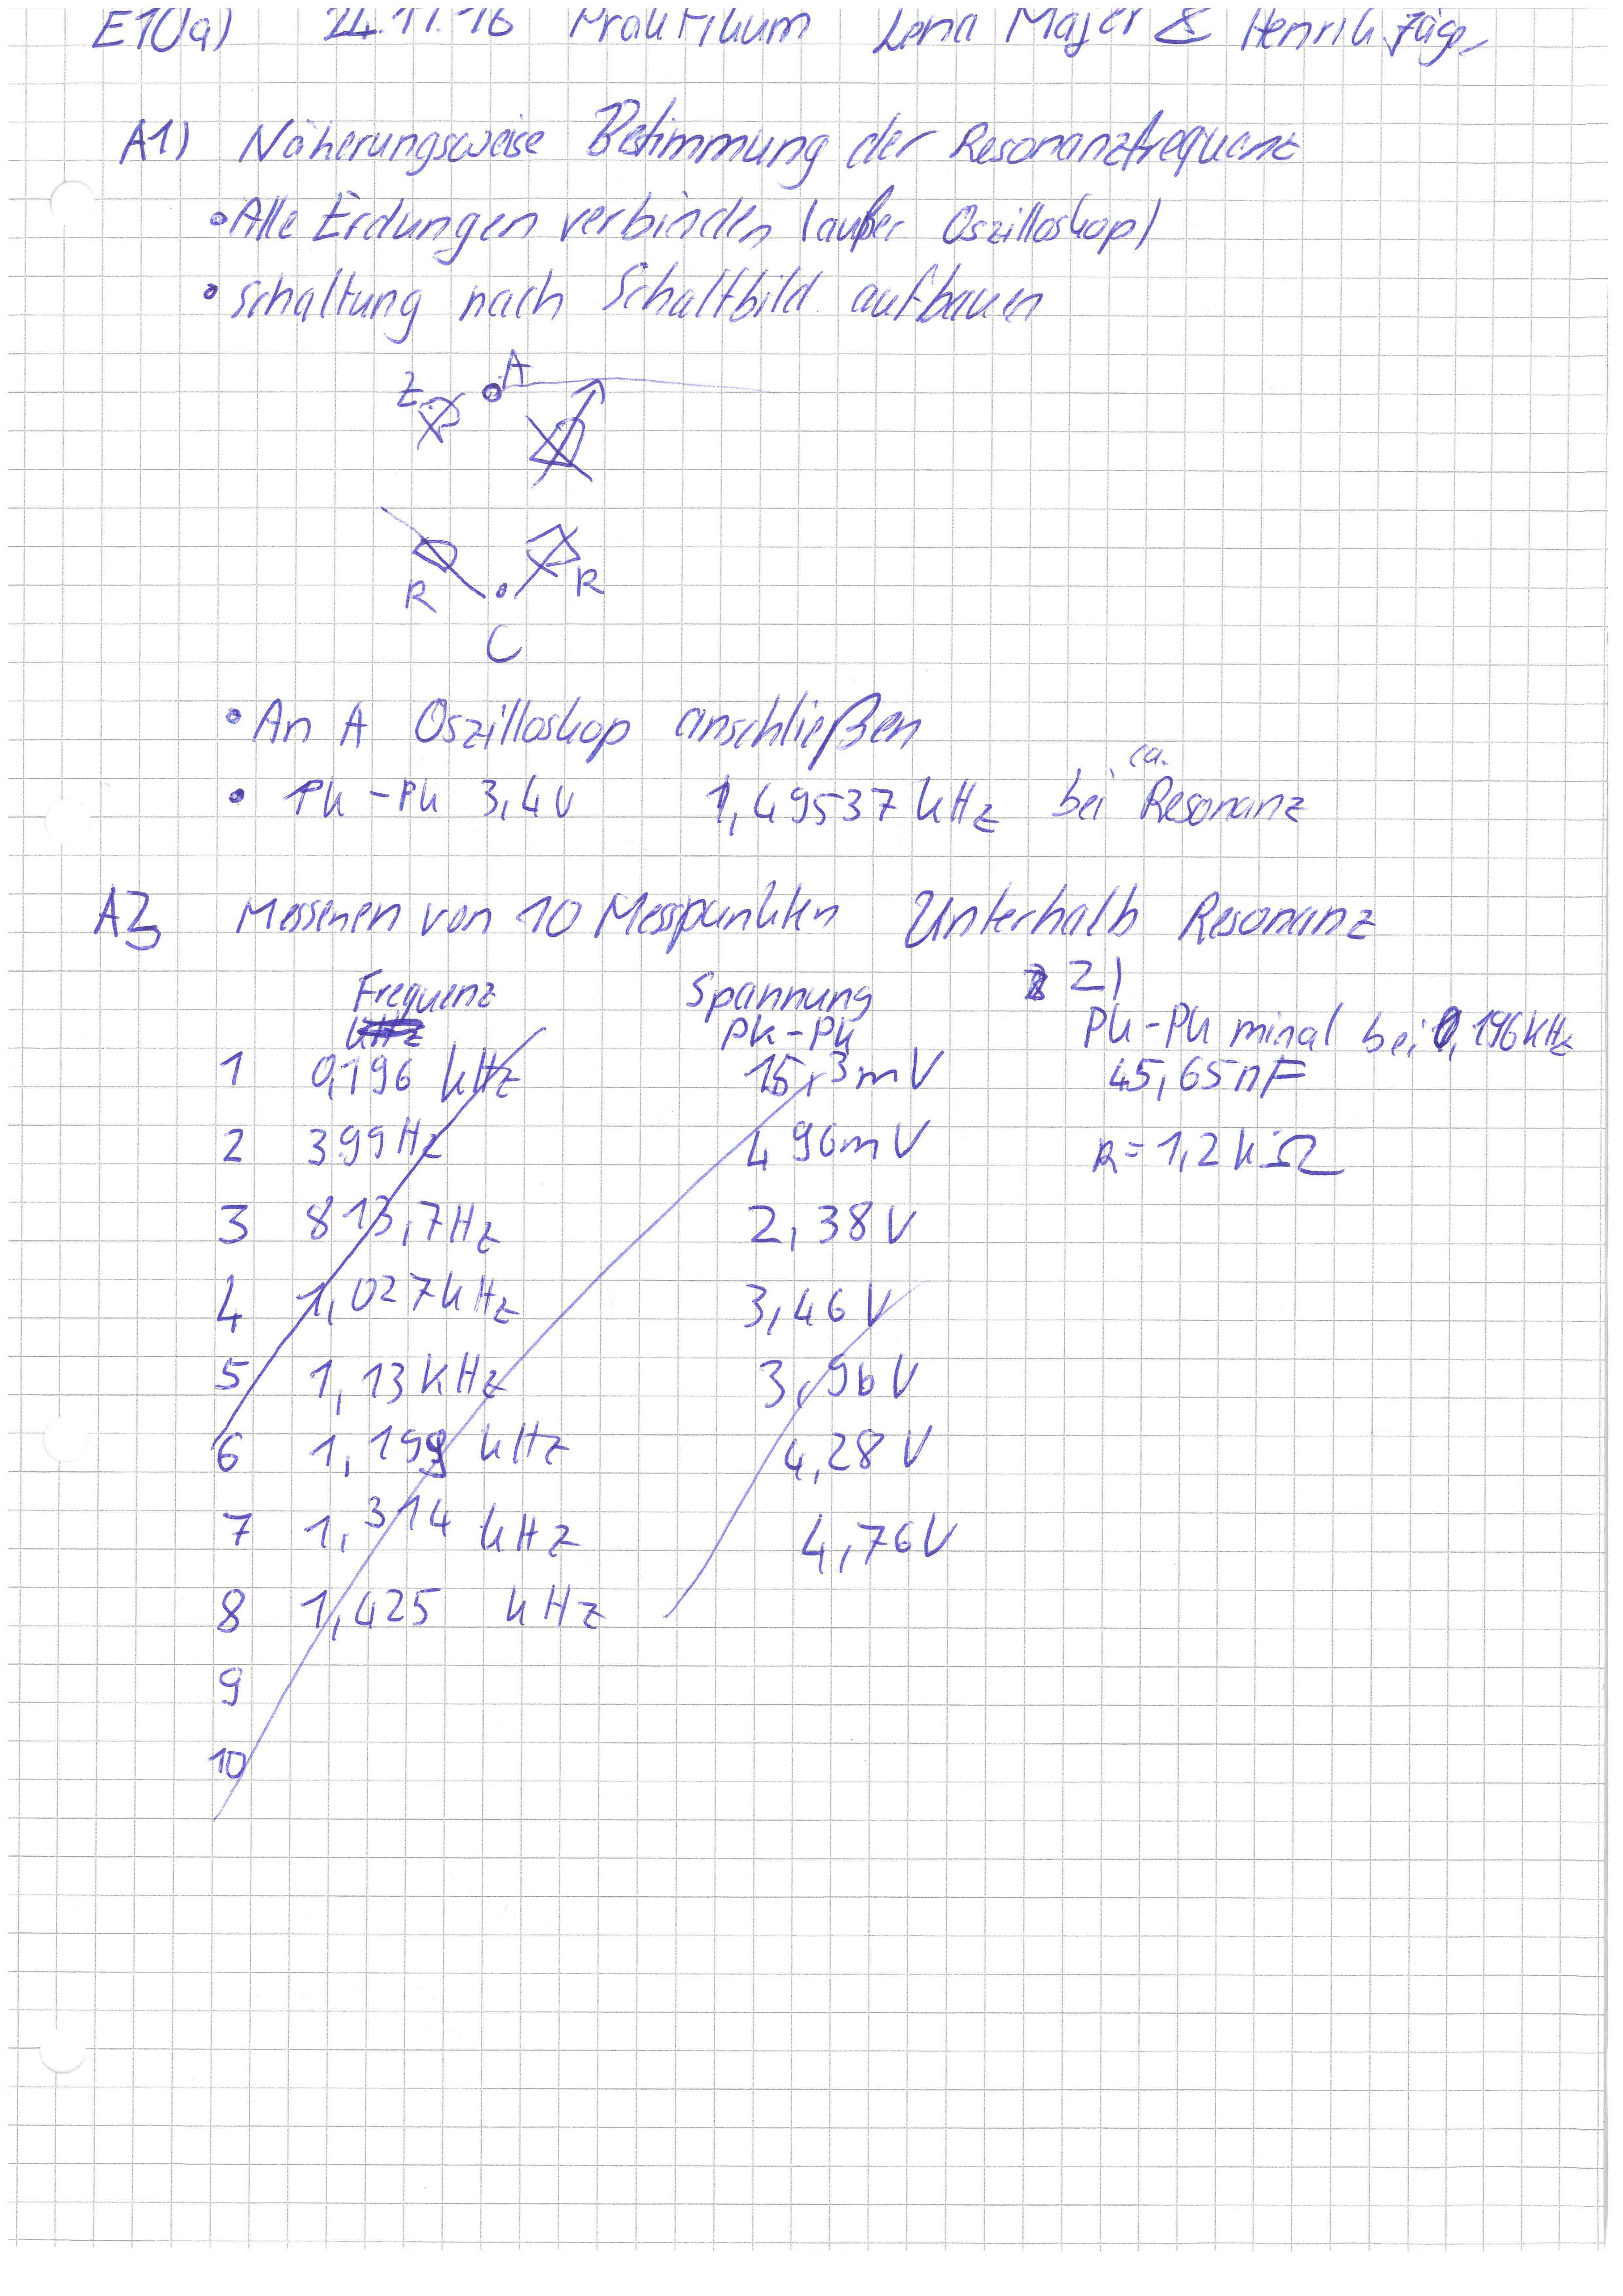
\includegraphics[scale=0.65]{Daten/1.jpg}
    	\end{center}
    	\captionof{figure}[Seite 1]{Messprotokoll Seite 1}
    	\pagebreak
    	
        \begin{center}
    		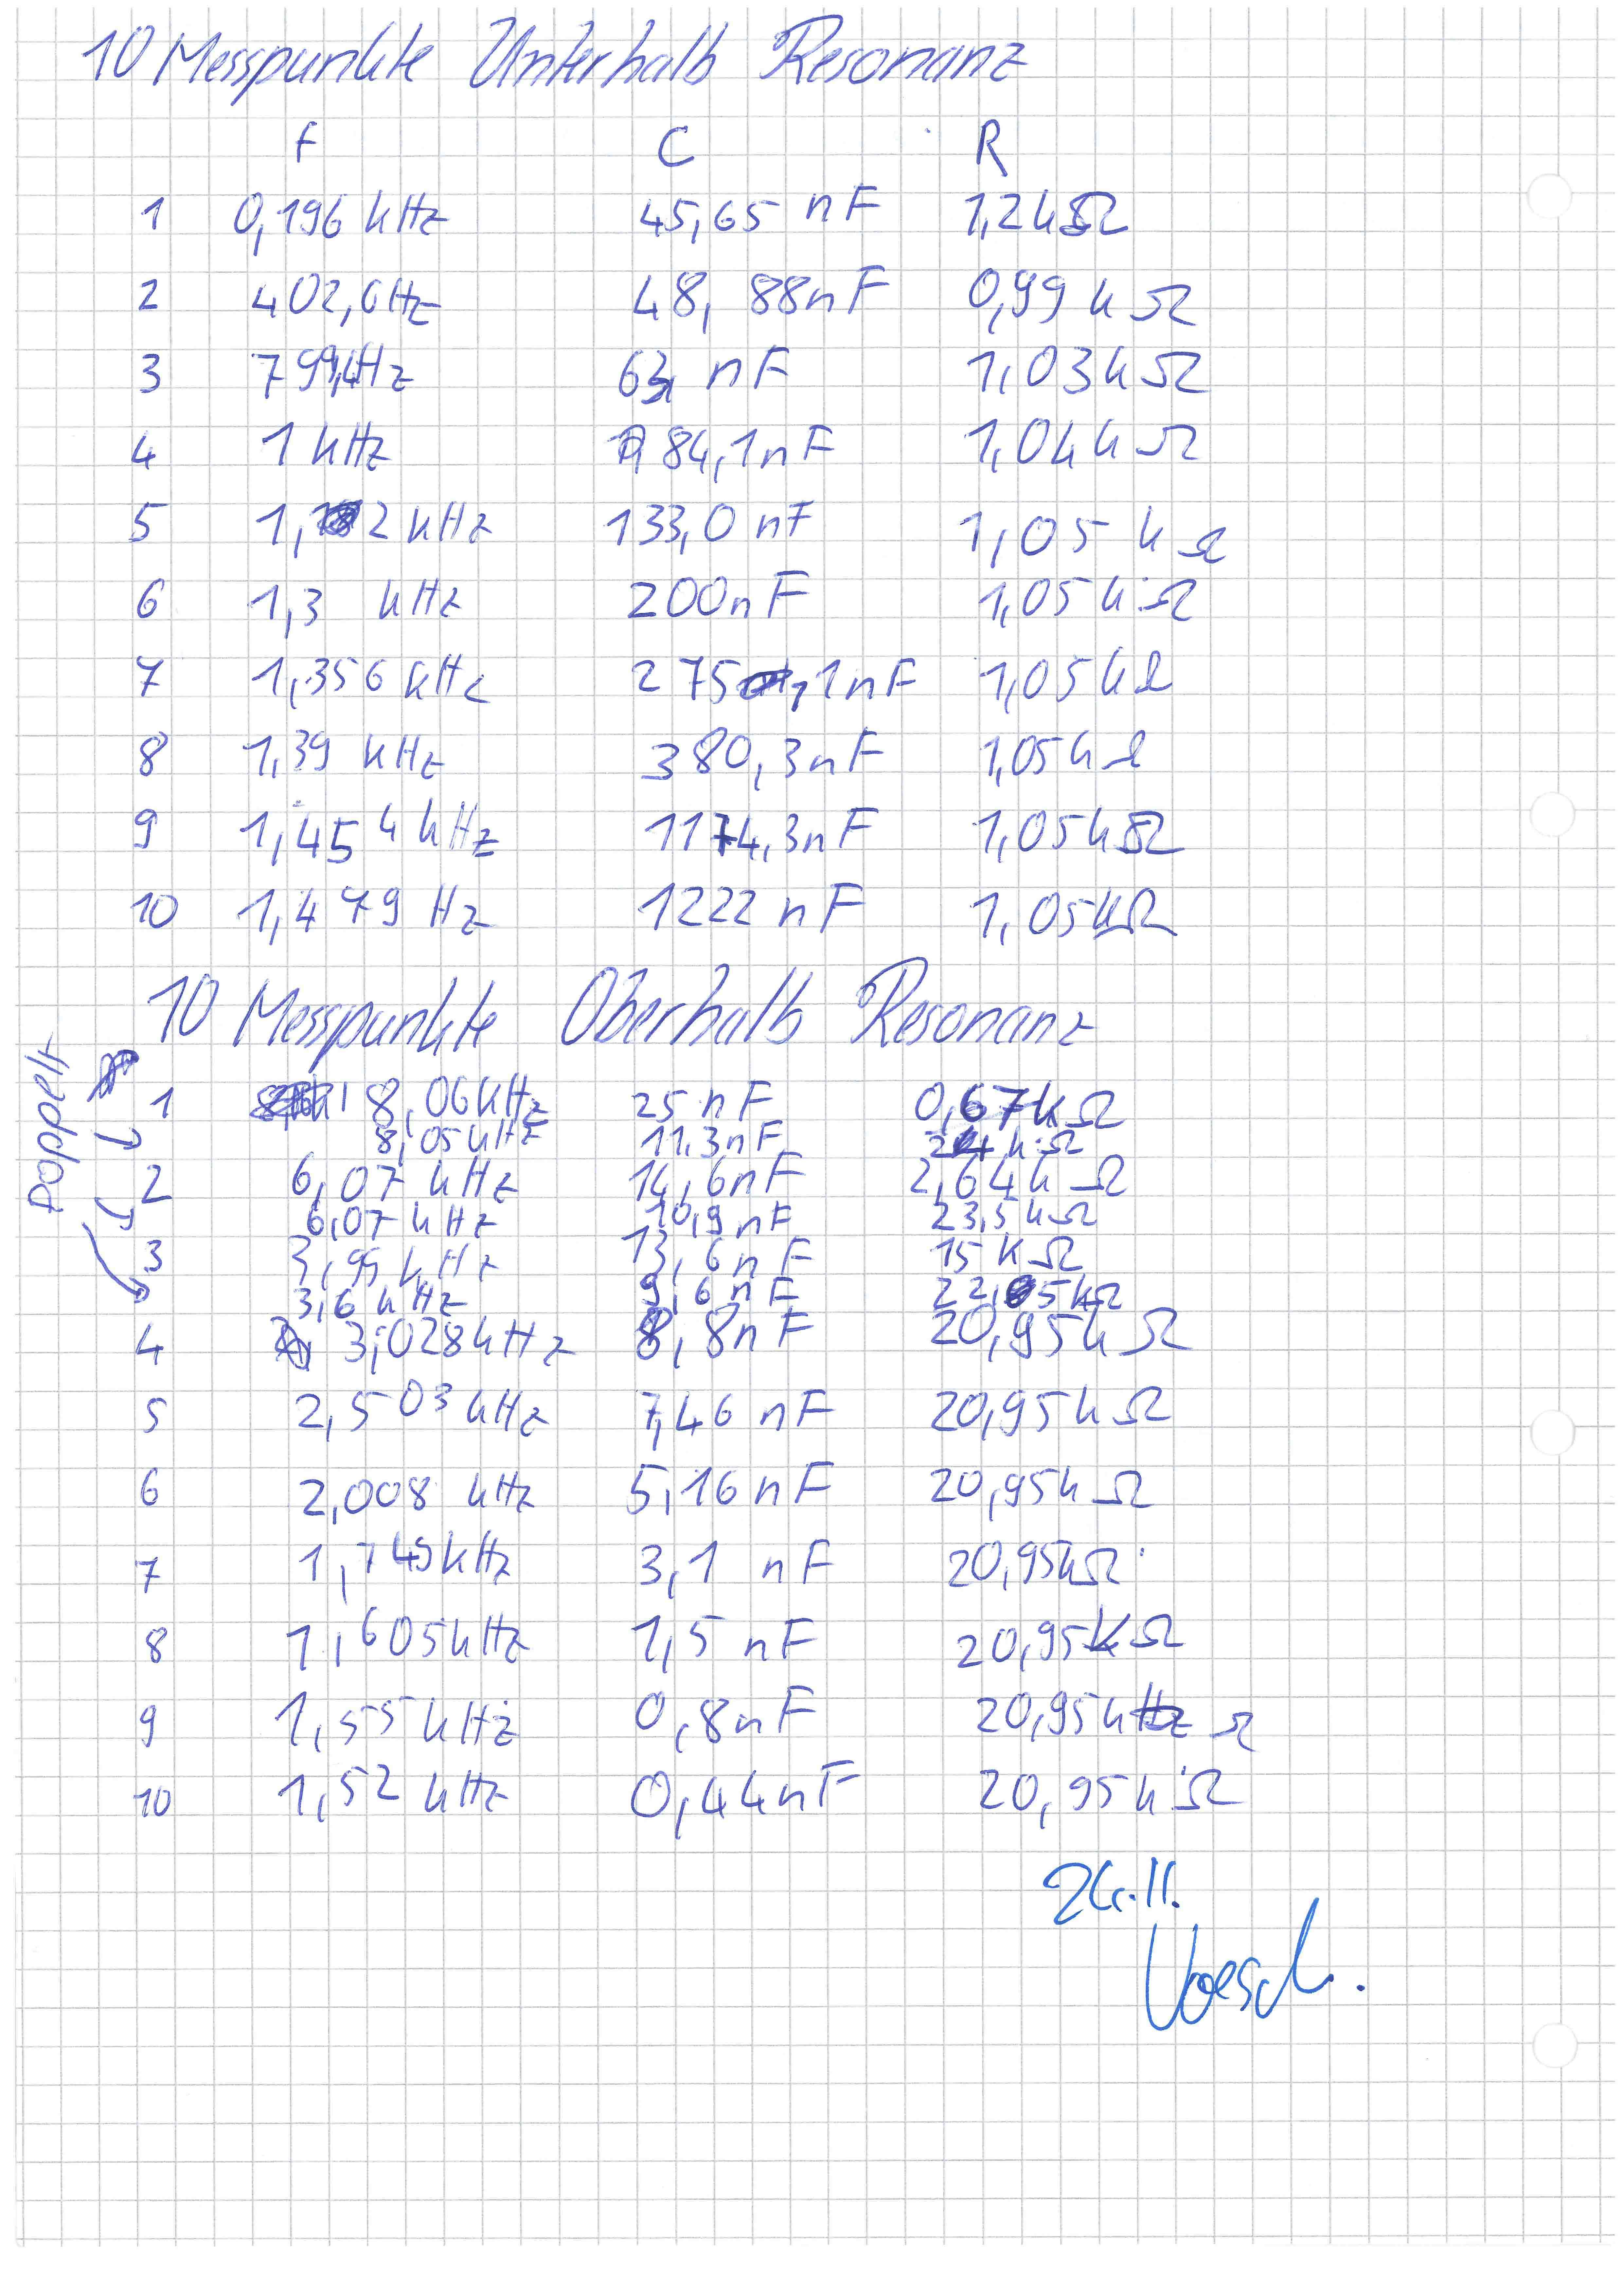
\includegraphics[scale=0.65]{Daten/2.jpg}
    	\end{center}
    	\captionof{figure}[Seite 2]{Messprotokoll Seite 2}
    	\pagebreak
	\pagebreak







\end{document}
